\chapter{Background}
\label{chapter:background} 



\section{DDoS attack and defense mechanisms}
\label{sec:BGDDoS}

A denial-of-service attack is characterized by an explicit attempt by attackers to prevent the legitimate users of a service from using that service~\cite{dosCert} provided by a network or server. There are two manner to launch this kind of attack. The first approach is overwhelm the network and occupy all the resources of a service sending massive volumes of useless traffic

\subsection{Protocol Attacks}



\subsection{Bandwidth Attacks}

\subsection{Logic Attacks}

\section{OpenFlow}
\label{sec:BGOpenFlow}

The explosion of mobile devices, server virtualization, security problems and advent of cloud service are among the reasons because the networking industry is beginning to question the traditional network architecture. OpenFlow is intended to solve the problem of assigning resources to users in a easy-way giving them the control plane of the network without disturbing the traffic flows. 

\par 

In traditional routers and switches, both control plane (high level routing decisions) and data plane (packet forwarding) are embedded in the same device. An OpenFlow Switch separates these two functions (Figure~\ref{fig:OpenFlowSwitch}). The data plane function still resides on the switch, while the control plane is moved to a separate device called Controller (see~\ref{subsec:OFController}) that manages the switch and communicates to each other over the Secure Channel (see~\ref{subsec:SCSecureChannel}) via the OpenFlow protocol (see~\ref{subsec:OFProtocolSC}).

\par 

\begin{figure}[htb]
\centering
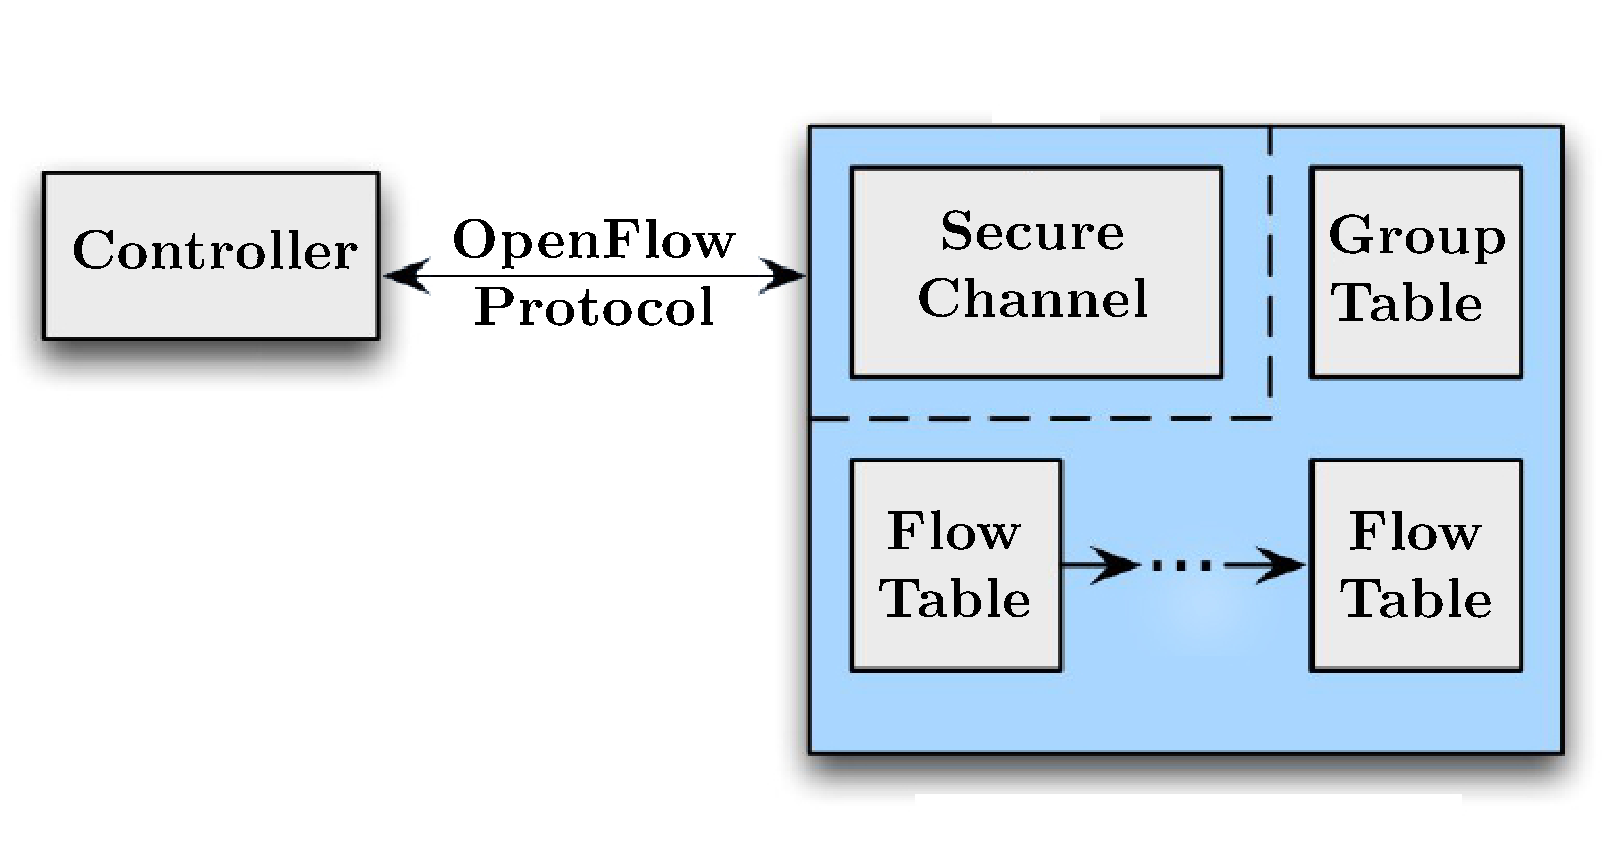
\includegraphics[width=0.8\textwidth]{./images/OpenFlowSwitch.pdf}
\caption{OpenFlow Switch components} \label{fig:OpenFlowSwitch}
\end{figure}

\par 

The switch contains \textit{flow tables} ~\ref{subsec:SCFlowTable}, which are updated through OpenFlow protocol adding, updating and deleting their \textit{flow entries}. When the flow traffic arrives to the switch, it checks if the arrived packets match in the flow table, if so, the action defined in the flow entry is executed. Otherwise, the packet is either sent it to the Controller or dropped.

\bigskip

Throughout this section, we will explain in detail the main parts of the OpenFlow Switch, as well as the Controller and how they work together. The first version of the OpenFlow (1.1) protocol was released on 2011, one year later, in February 2012, the ONF approved and published the version 1.2. Nowadays, the current version of the protocol and the one that will be used in this project is the 1.4 ~\cite{OpenFlowSpecification}.

\subsection{Switch Components}
\label{subsec:PFSwitchComponents}

\subsubsection{Flow Table}
\label{subsec:SCFlowTable}

\begin{table}[h]
\centering
\begin{tabular}{ | c | c | c | c | c | c | }
  \hline                       
  Match Fields & Priority & Counters & Instructions & Timeouts & Cookie \\
  \hline  
\end{tabular}
\caption{Main components of a flow entry}
\end{table}


\begin{table}[h]
\centering
\begin{tabular}{ | c | c | c | c | c | c | c | c | c | c | c | c | }
  \hline                       
  \begin{sideways}Ingress Port\end{sideways} &\begin{sideways}Ether source\end{sideways}  &\begin{sideways}Ether dst\end{sideways}  &\begin{sideways}Ether type\end{sideways}  &\begin{sideways}VLAN id\end{sideways}  &\begin{sideways} VLAN priority\end{sideways} &\begin{sideways}IP src\end{sideways}  &\begin{sideways}IP dst\end{sideways}  &\begin{sideways}IP proto\end{sideways}  &\begin{sideways}IP ToS bits\end{sideways}  &\begin{sideways} src port\end{sideways} &\begin{sideways}dst port\end{sideways}  \\
  \hline  
\end{tabular}
\caption{Main components of the Match Field}
\end{table}

\begin{sideways}\end{sideways}

\subsubsection{Secure Channel}
\label{subsec:SCSecureChannel}

\subsubsection{OpenFLow Protocol}
\label{subsec:OFProtocolSC}

\subsection{Controller}
\label{subsec:OFController}

\section{POX}
\label{sec:BGPOX}
